\section{Resultados e discussão: RQ05 e RQ06}
\label{sec:resultados-b}

As análises utilizam uma observação por repositório, sem ponderação por número
de commits ou runs. Os 11 CFR(b) indisponíveis e os 22 tempos de recuperação
ausentes não são imputados: os denominadores são 300, 289 ou 278, conforme a
métrica. Nos 22 casos não houve episódio observável, o que não significa
recuperação instantânea. Os 90 episódios censurados, dentre 7.861, permanecem
registrados; as medianas de recuperação utilizam apenas episódios concluídos.

\subsection{RQ05: frequência e falhas}

Calculamos Spearman bilateral para cada proxy. Como diferencial, estimamos
intervalos de confiança de 95\% por bootstrap BCa pareado e p-valores por
permutação dos pareamentos, ambos com 9.999 reamostragens e semente 42. A
recomendação de conferir o p-valor assintótico em amostras menores está na
documentação do SciPy~\cite{scipySpearman,scipyBootstrap}. Holm corrige a família
dos dois p-valores de permutação, mantendo os p-valores originais de Spearman.

\begin{table}[htbp]
\centering\footnotesize
\caption{RQ05: associações e incerteza. Última coluna: permutação após Holm.}
\label{tab:rq05}
% Gerado por analises.sprint3_b
\begin{tabular}{lrrrr}
\hline
Proxy & $n$ & $\rho$ [IC 95\%] & $p$ Spearman & $p$ perm./Holm \\
\hline
CFR (a) & 300 & 0,015 [-0,095; 0,125] & 0,7993 & 0,8096 \\
CFR (b) & 289 & 0,660 [0,585; 0,724] & $1,48\times 10^{-37}$ & 0,0004 \\
\hline
\end{tabular}

\end{table}

O CFR de CI apresenta associação próxima de zero ($\rho=0{,}015$), com IC que
inclui zero. Para o CFR de entrega, a associação é positiva ($\rho=0{,}660$),
com IC de 0,585 a 0,724. A Figura~\ref{fig:rq05} preserva os CFR iguais a zero;
apenas a frequência usa escala logarítmica. O p-valor por permutação tem resolução
finita, portanto seu valor pequeno não é apresentado como zero.

\begin{figure}[htbp]
\centering
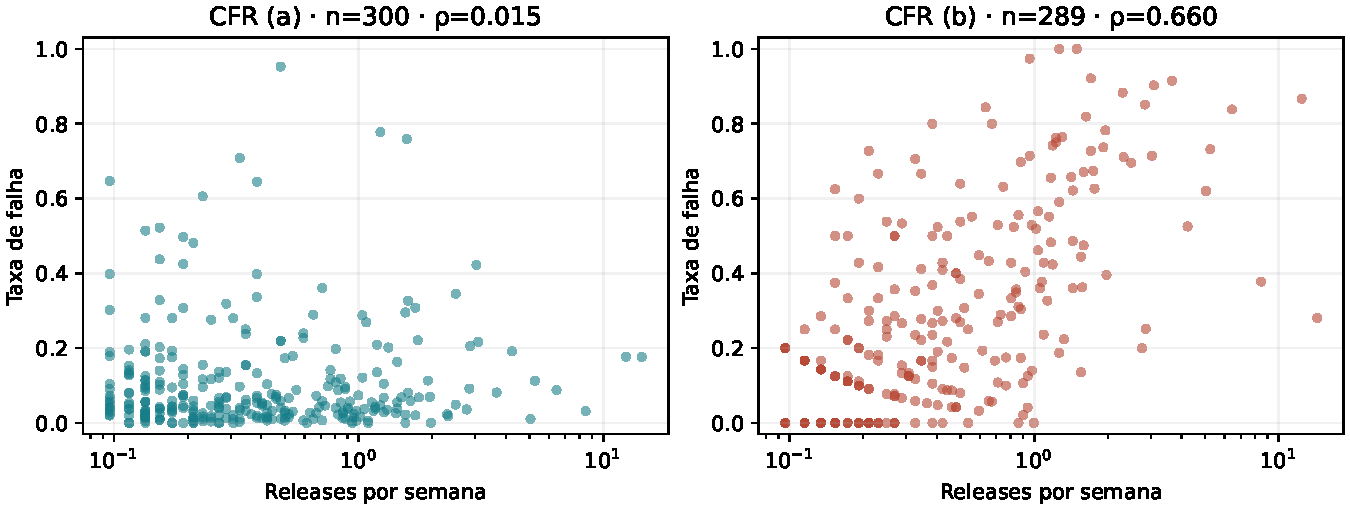
\includegraphics[width=\textwidth]{../../results/s03_b/rq05_dispersao.pdf}
\caption{Frequência de releases e os dois proxies de falha. Cada ponto é um projeto.}
\label{fig:rq05}
\end{figure}

Retirar um projeto por vez mantém o sinal das duas correlações. O $\rho$ de CI
varia entre 0,006 e 0,024; o de entrega, entre 0,657 e 0,668. As maiores alterações
absolutas são 0,0093 e 0,0076, respectivamente. A associação positiva de entrega
não depende de um único repositório; isso não resolve vieses compartilhados
pela amostra ou pela definição operacional.

\textbf{H5 não é sustentada}: esperava-se associação fraca e negativa. Não
encontramos evidência de associação monotônica no proxy de CI, enquanto o de
entrega associa maior frequência a maior CFR. Esse resultado não contradiz
diretamente a evidência DORA sobre produção: nossos eventos são proxies.
Uma explicação metodológica possível é que publicar mais releases cria mais
oportunidades de encontrar uma corretiva nos sete dias seguintes. A associação
pode refletir esse acoplamento, além de diferenças reais entre projetos; o estudo
não identifica a contribuição causal de cada mecanismo.

\subsection{RQ06: tipo, comunidade e linguagem}

Escolhemos os três fatores ligados à H6. Os quartis de contribuidores têm
limites 1, 23, 55,5, 125,5 e 1.963, preservando empates: os grupos possuem
76, 74, 75 e 75 projetos. Linguagens com menos de dez projetos formam
``Outras'' (67 projetos), resultando em nove grupos. Os quatro tipos originais
são mantidos. Grupos são fixados antes das exclusões por métrica.

Aplicamos Kruskal--Wallis às 18 combinações dos três fatores com frequência,
lead time (a)/(b), CFR (a)/(b) e recuperação. O código também contempla dois
grupos com Mann--Whitney e Cliff's $\delta$; esse caso não ocorre na amostra.
Reportamos $\varepsilon^2=H/(n-1)$ e corrigimos conjuntamente os 18 p-valores
por Holm ($\alpha=0{,}05$). Mediana, Q1, Q3, IQR, tamanhos dos grupos,
ausências e os 18 resultados completos estão nos CSVs reproduzíveis.

\begin{table}[htbp]
\centering\footnotesize
\caption{RQ06: seis comparações com p ajustado menor que 0,05, de 18 realizadas.}
\label{tab:rq06}
% Gerado por analises.sprint3_b
\begin{tabular}{llrrr}
\hline
Fator & Métrica & $n$ & $p$ Holm & $\varepsilon^2$ / $\delta$ \\
\hline
Tipo do projeto & Recuperação & 278 & 0,0347 & 0,051 \\
Contribuidores (quartis) & Lead time (a) & 300 & $8,10\times 10^{-7}$ & 0,124 \\
Contribuidores (quartis) & Lead time (b) & 300 & $6,11\times 10^{-9}$ & 0,157 \\
Contribuidores (quartis) & Recuperação & 278 & 0,0092 & 0,062 \\
Linguagem & Lead time (a) & 300 & 0,0002 & 0,124 \\
Linguagem & Lead time (b) & 300 & 0,0199 & 0,084 \\
\hline
\end{tabular}

\end{table}

A comunidade de contribuidores se associa aos dois lead times e à recuperação;
a linguagem, aos dois lead times; e o tipo, à recuperação. Não encontramos
evidência ajustada de diferenças em frequência ou CFR por esses fatores.
A magnitude dos efeitos observados consta na Figura~\ref{fig:rq06}; significância
não equivale a relevância prática, e grupos de composições distintas não permitem
um ranking causal dos fatores.

\begin{figure}[htbp]
\centering
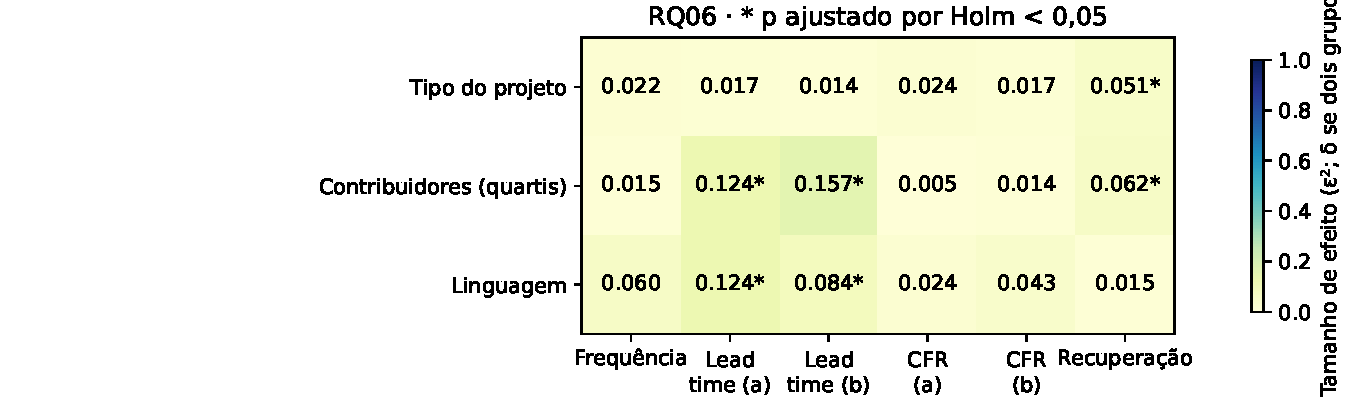
\includegraphics[width=\textwidth]{../../results/s03_b/rq06_efeitos.pdf}
\caption{RQ06: tamanho de efeito nas 18 comparações; asteriscos indicam Holm $<0{,}05$.}
\label{fig:rq06}
\end{figure}

\textbf{H6 recebe apoio parcial}. Contribuidores apresentam associações, mas
comunidades maiores não exibem os tempos menores esperados: o lead time (b)
mediano passa de 53,95 horas no Q1 (Q1--Q3: 20,24--196,94) a 421,34 horas no Q4
(170,68--1.285,34). A recuperação mediana é 0,70 hora no primeiro quartil
(0,39--6,71) e 4,62 horas no último (2,07--20,94). A linguagem também apresenta
associações, e o tipo não distingue a frequência após o ajuste. Esses contrastes
são descritivos: o teste global não identifica quais pares diferem, e não foram
realizados testes post-hoc. Complexidade, idade e políticas de publicação podem
confundir essas relações.

\subsection{Limites das conclusões desta etapa}

Bootstrap, permutação e análise de influência quantificam estabilidade
condicionada à amostra, sem corrigir seleção, ausência potencialmente informativa
ou erros da heurística. O grupo ``outro'' possui apenas seis recuperações
observadas. O tipo provém de consenso triplo em 60 projetos e revisão individual
após sugestões automáticas em 240. A amostra cobre projetos com 1.000 a 8.000
estrelas, e a heurística foi refinada e avaliada na mesma amostra-ouro. Essas
limitações impedem generalização automática para produção ou para todo o GitHub.
A análise de sensibilidade da RQ07 será necessária para avaliar mudanças de
definição operacional; a estabilidade individual aqui medida não a substitui.
